% IEICE Infromation Theory Conference (Technical Meeting)
% Template for the IEICE technical report
% Size: A4 (not US Letter)
% Page: at most 6

\documentclass[twocolumn]{article}

%%% Do not change page parameters
\usepackage{techrep}
\usepackage{amsfonts}
\usepackage{amssymb}
\usepackage{eufrak}
\usepackage{csvsimple}
\usepackage{caption}
\usepackage{longtable}
\usepackage{amsmath}
\usepackage{bm}
\usepackage {graphicx}
\usepackage {graphics}
\setlength{\columnsep}{10mm}
\setlength{\textwidth}{180mm}
\setlength{\textheight}{250mm}
\addtolength{\oddsidemargin}{-9mm}
\addtolength{\topmargin}{-25mm}
\newtheorem{theorem}{Theorem}[section]
\newtheorem{corollary}{Corollary}[theorem]
\newtheorem{lemma}[theorem]{Lemma}
\newtheorem{example}[theorem]{Example}
%%%

\title{How to Prepare and Submit Papers}
\author{
Hanako DENSHI${}^{\dagger}$,
Taro JOHO${}^{\ddagger}$,
and Jiro TSHUSHIN${}^{\dagger}$}
\date{
\begin{tabular}{c}
 ${}^{\dagger}$
 Faculty of Engineering, First University \\
 Yamada 1-2-3, Minato-ku, Tokyo, 105-0123 Japan\\
 ${}^{\ddagger}$
 R\&D Division, Osaka Corporation \\
 Kawada 4-5-6, Suita-shi, 565-0456 Japan
\end{tabular}
}


\begin{document}

\begin{abstract}
 IEICE (The Institute of Electronics, Information and Communication Engineers)
 provides a template file for the IEICE Technical Report.
\end{abstract}

\begin{keyword}
 IEICE, IEICE technical report, \LaTeX, template
\end{keyword}

\maketitle


\section{Introduction}
The construction of a turbo code is usually done by the parallel concatenation of two
convolutional codes via an interleaver. The good BER performance of turbo codes at
low SNR  is attributed to the interleaver, which effectively thins the distance spectrum
of the turbo code [distance spec interp]. Due to its importance, extensive research has
been conducted on interleavers for turbo codes. Interleavers for turbo codes are 
generally grouped into random and deterministic interleavers. The most common 
random interleaver can be achieved by rearranging elements in an alphabet in
pseudo-random fashion. This interleaver was used in [4] and 
was shown to achieve performance very close to the Shannon limit for long frame 
sizes. 
\paragraph{}
The disadvantage associated with random interleavers arises from the necessity of 
storing interleaver tables in both the encoder and decoder. For applications were 
large interleaver sizes are required, the memory requirements to store the interleaver
tables alone makes the use of these interleavers undesirable.  Deterministic interleavers
are a solution to necessity of interleaver tables as the interleaving is done via 
algorithm. Deterministic interleavers are being used in many applications, most 
notably the Quadratic Permutation Polynomial (QPP) Interleaver [5] which is used 
in 4G LTE applications.
\paragraph{}
The most basic deterministic interleavers are the linear and block interleavers [2]
The index mapping function of the linear interleaver is 
$$ \Pi_{\mathfrak{L}_N}(i) \equiv di \mod N \,\,\,\,\, 0 \leq i < N, \, gcd(N,d)=1$$
The design of the linear interleaver is essentially picking a suitable value of d for a
given interleaver length N and in [2] considerations for choosing a suitable 
value for d is introduced. For long frame sizes, linear interleavers perform worse
than random interleavers due to prescence of a high error floor. Many other 
deterministic interleavers have been proposed, including the quadratic interleaver
[2] which performs well but not as good as the random interleavers for long
interleaver frame sizes. 

\paragraph{}
In this paper, we design our interleaver by reviewing the linear interleaver and making
a slight modification to it to improve its performance.

\section{Turbo Codes:Review}
In this section, we review the encoding and decoding process for turbo codes for BPSK
modulation and transmission over the AWGN channel.
	
\subsection{Turbo Encoding}

\begin{figure}[h!]
\centering
		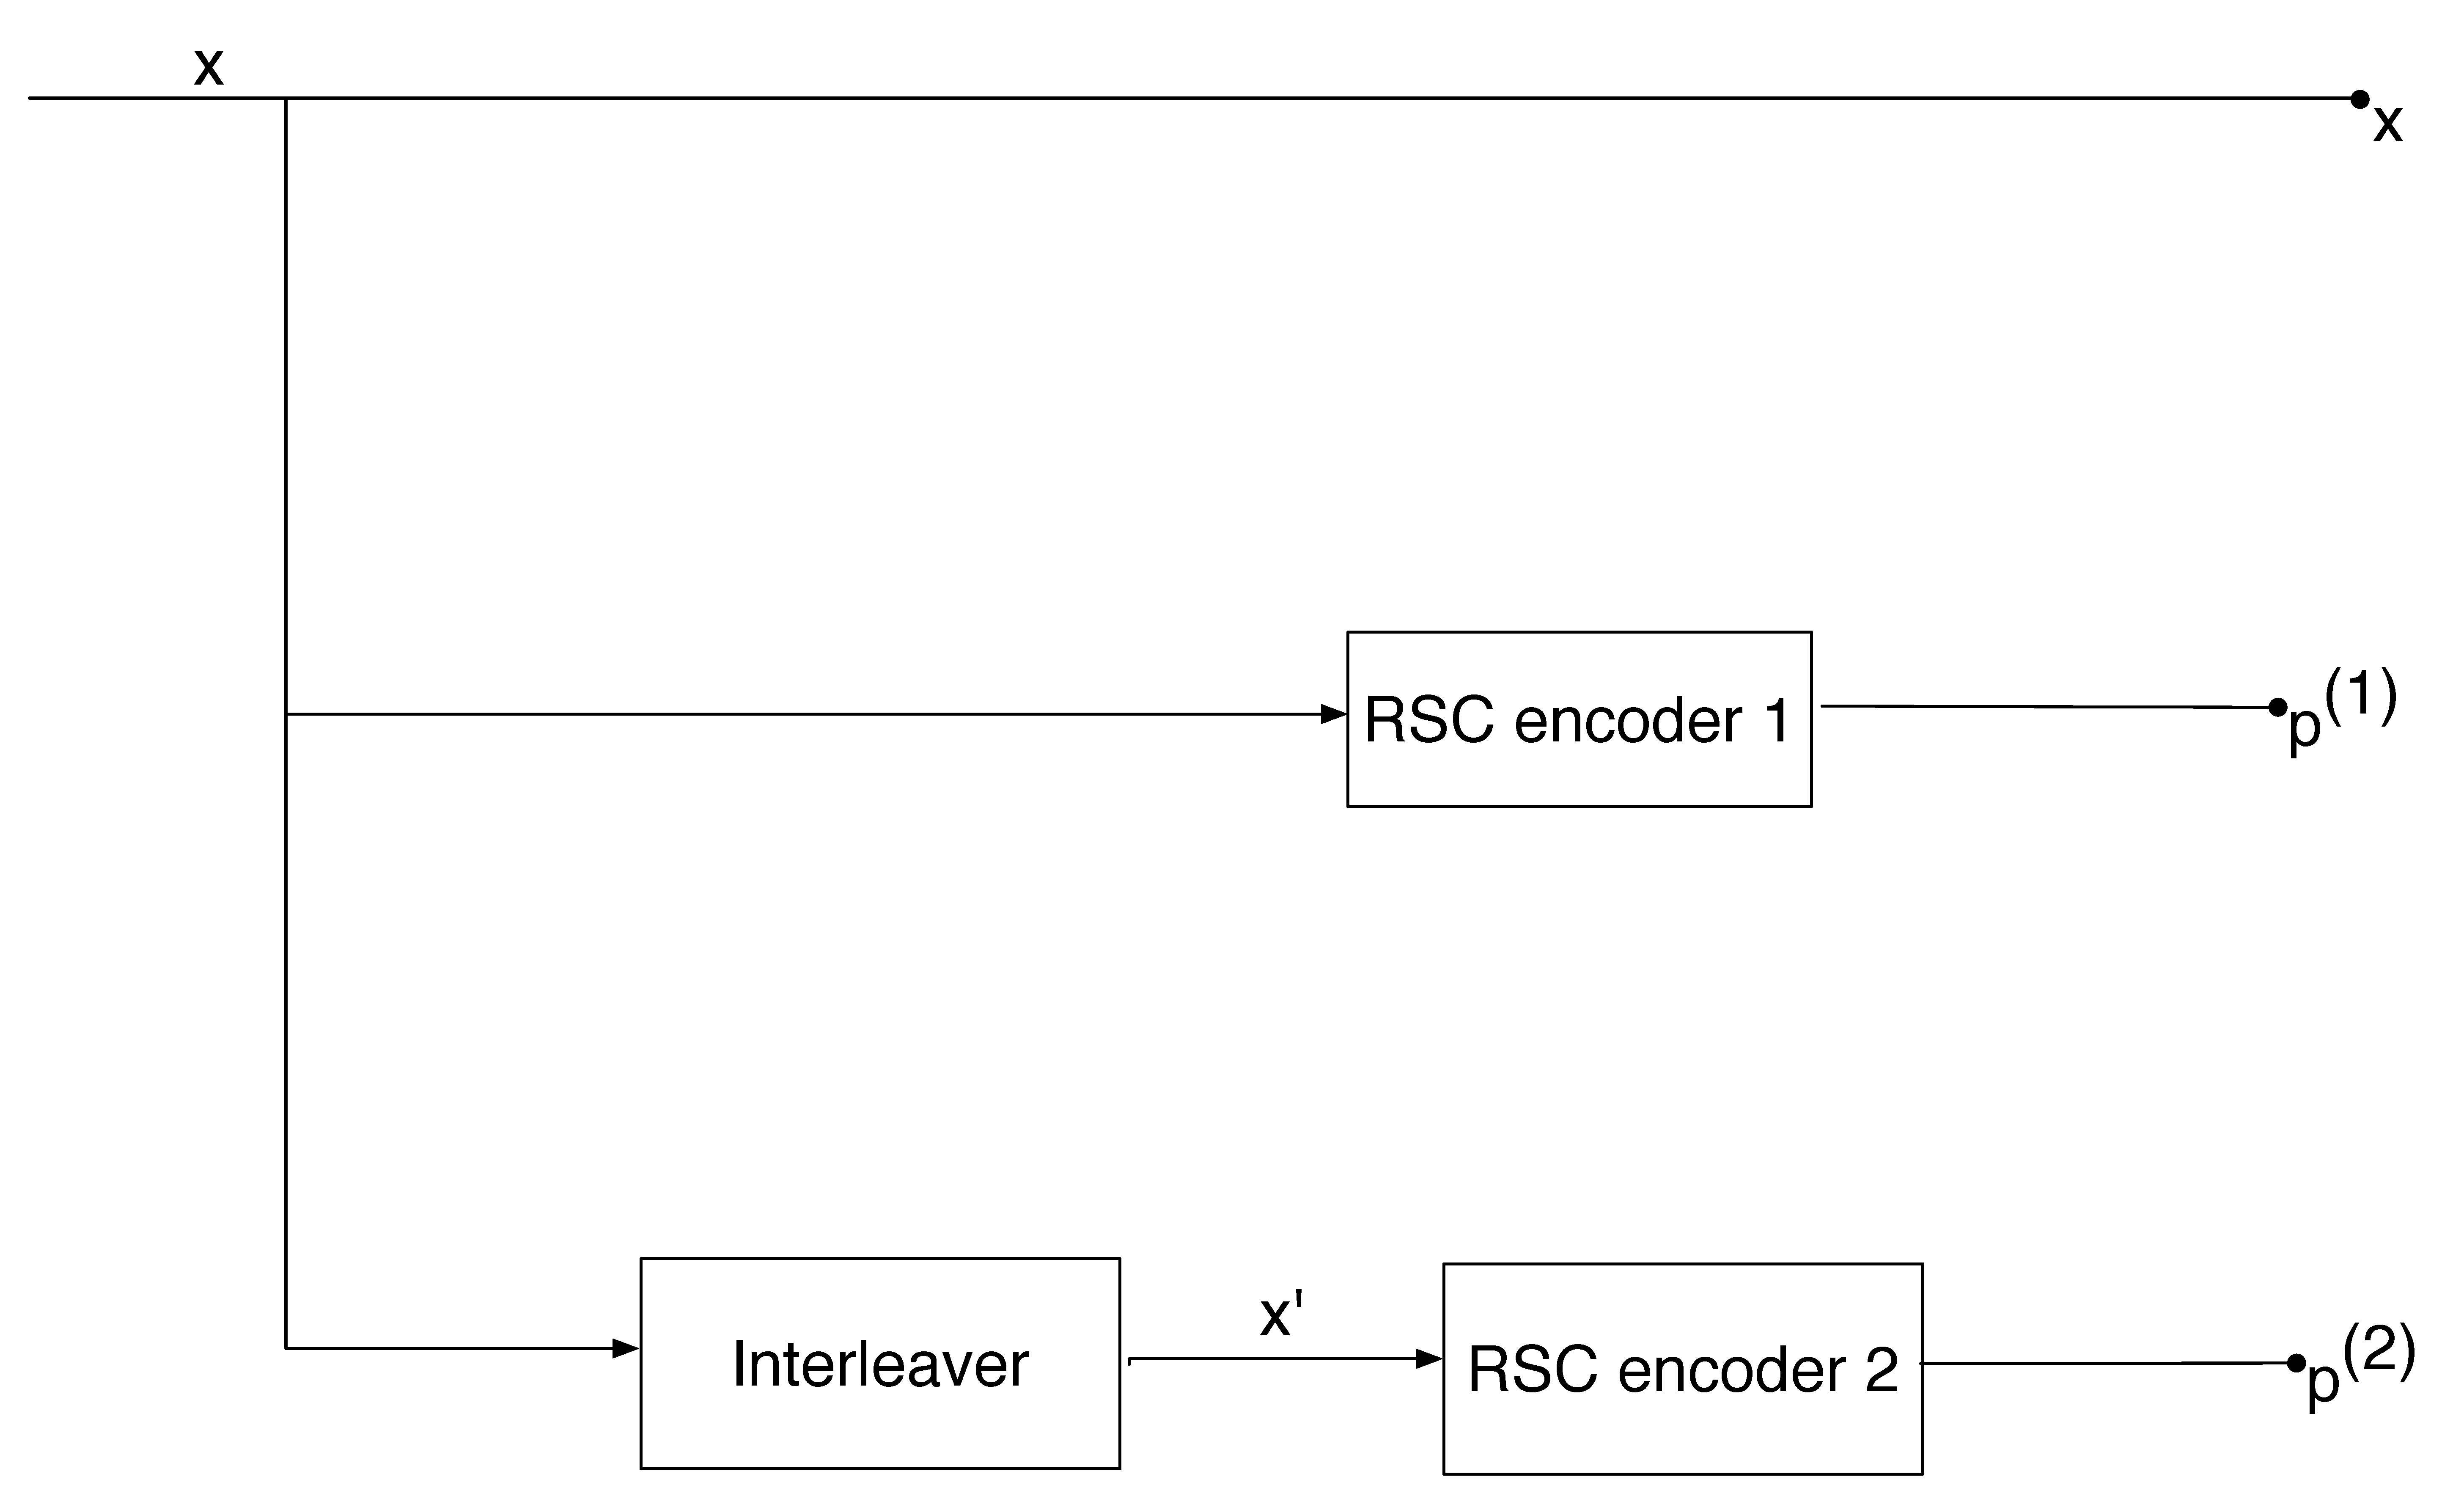
\includegraphics[width=0.5\textwidth]{TurboEncoder.pdf}
		\caption{Turbo Encoder}
		\label{TC}
		\end{figure}
	
\paragraph{}The system diagram for the turbo encoder is shown in figure(\ref{TC}).
 It is made up of identical Recursive Systematic Convolutional (RSC) encoders which 
 are connected
  in parallel via an interleaver. The RSC encoders have constraint length K and output
  n bits for every k bits input at time t.
  From here onward we refer to the RSC encoders as component 
encoders (CE). The generator matrix of the component codes are written in 
the form $[1 \frac{F(D)}{H(D)}]$ or simply as $[\frac{F(D)}{H(D)}]$
where the numerator and the denomenator represent the feedfoward and feedback
 connections of the component encoder. The $''1''$ represents the information 
 (systematic) bits fed into the encoder.

 The generator matrix for the one shown in figure (\ref{RSC})
 is $[\frac{1+D^2}{1+D+D^2}]$ .The encoding process is as follows.

\begin{figure}[h!]
\centering
		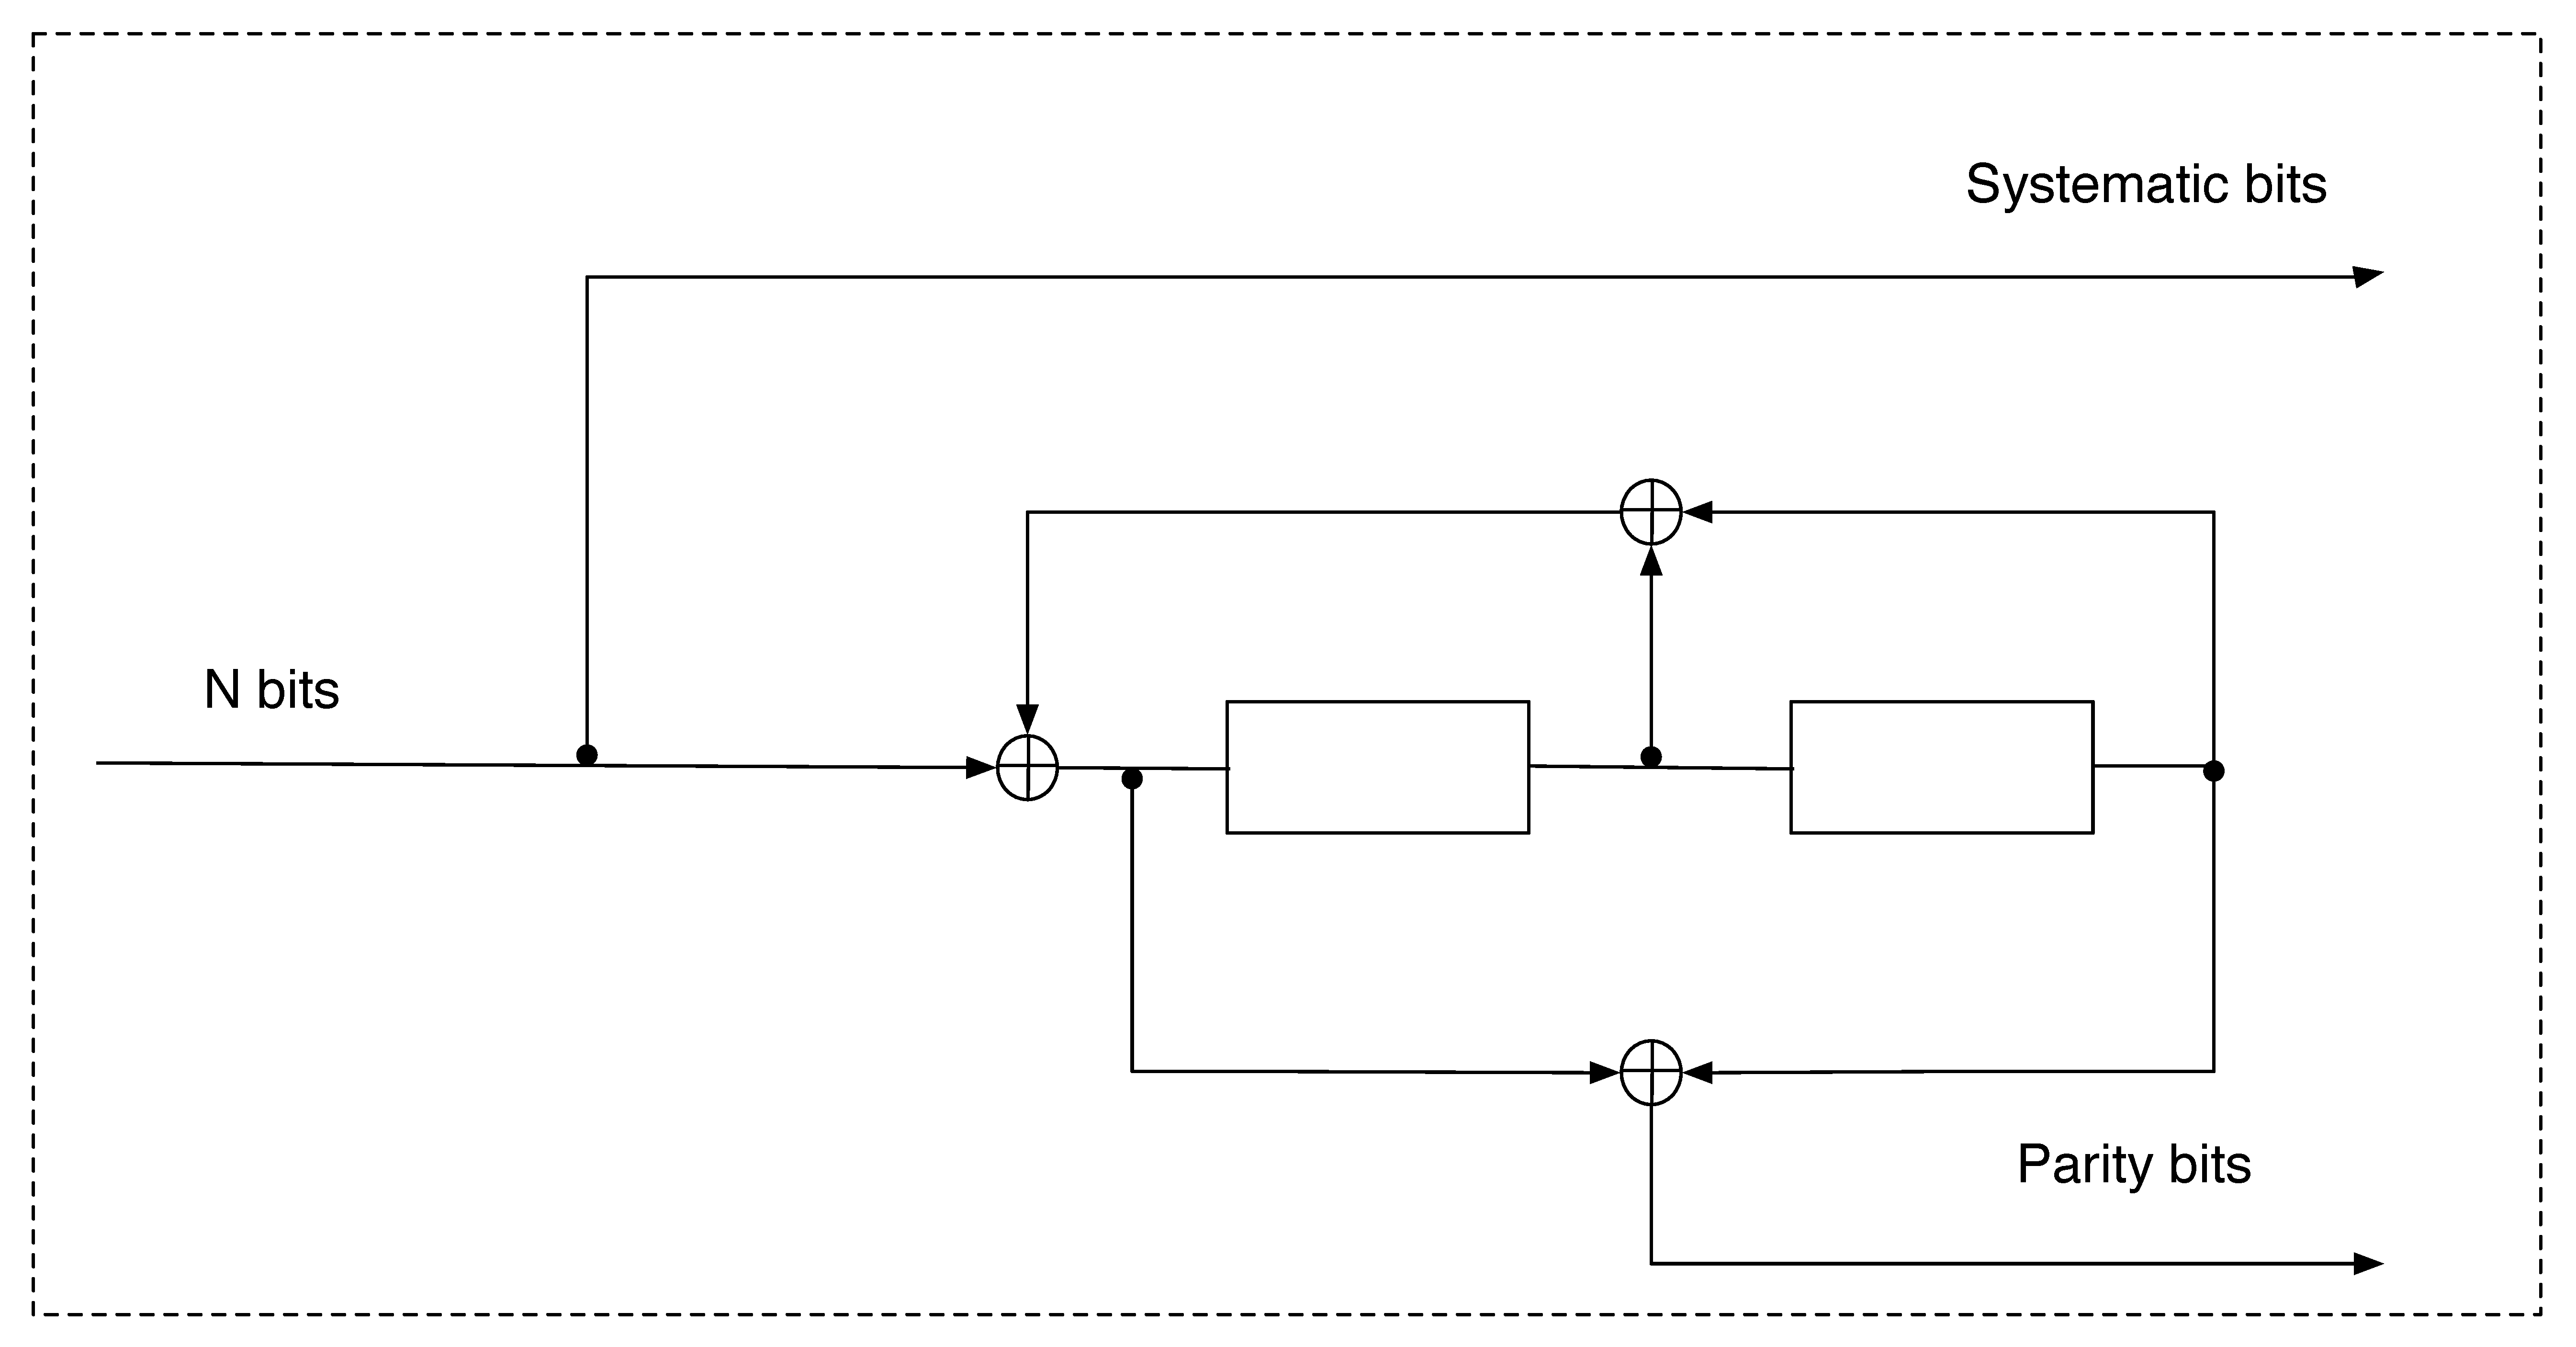
\includegraphics[width=0.45\textwidth]{RSCExample3.pdf}
		\caption{$[\frac{1+D^2}{1+D+D^2}]$  RSC Encoder}
		\label{RSC}
		\end{figure}

\paragraph{}
In our encoding scheme, we terminate the CE1 and leave CE2 open. This is done due
to the difficulty involved in terminating both CE1 and CE2 with the same tail bit 
sequence.
To acheive this,	
 an information sequence $\mathbf{x}=\{x_0,x_1,...,x_{N-m-1} \} $
$m=K-1$
of length $N-m$ is fed into the turbo encoder. This is fed directly into CE1 (assumed to 
begin in the all-zero state) and produces the upper parity sequence 
$\mathbf{p}^{(1)}=\{p^{(1)}_0,p^{(1)}_1,...,p^{(1)}_{N-m-1} \}$ also of 
length $N-m$. 
Since it is desired to return CE1 to the all-zero state, $m$ extras tail bits 
are fed into CE1 which brings the total length of $p^{(1)}$ to $N$. The tail bits are
also added to $\mathbf{x}$ transforming it into a vector of length $N$.
The input to the CE2 (also assumed to 
begin in the all-zero state) is 
$\mathbf{x'}=\Pi(\mathbf{x})= \{x'_0,x'_1,...,x'_{N-1} \} $. This produce the lower 
parity sequence 
$\mathbf{p}^{(2)}=\{p^{(2)}_0,p^{(2)}_1,...,p^{(2)}_{N-1},...,p^{(2)}_{L-1} \}$
 which has total length $L=N+m$ due to the extra tail bits added to force CE2 back to the
 all-zero state. Since we wish to keep the trellis of CE2 open, we do not transmit the
 extra $m$ tail bits and the length of $\mathbf{p}^{(2)}$ is reduced to $N$.
 $\mathbf{x}$ (along with the extra m tail-bits), $\mathbf{p}^{(1)}$
 and $\mathbf{p}^{(2)}$ are multiplexed, BPSK modulated and transmitted over the
 AWGN channel.
 The turbo codeword generated  
 $$\mathbf{c}=\{x_0,p^{(1)}_0,p^{(2)}_0,...,x_{N-1},p^{(1)}_{N-1},p^{(2)}_{N-1} \} $$ 
 has length $3N$ and the
 turbo encoder has rate $R_c=\frac{N}{3N} = \frac{1}{3}$
 
 
 \subsection{Turbo Decoding}
 The turbo code transmitted over the AWGN channel is received by the turbo decoder as
  $\mathbf{y}=\{\mathbf{y}^x,\mathbf{y}^{p^{(1)}},\mathbf{y}^{p^{(2)}}\}$ 
  of length $3N$, where $\mathbf{y}^x,\mathbf{y}^{p^{(1)}},\mathbf{y}^{p^{(2)}}$
    correspond to the systematic, upper and lower parity sequence respectively.
    $$\mathbf{y}^x=\{y^x_0, y^x_1,...,y^x_{N-1}\}$$ 
    $$\mathbf{y}^{p^{(1)}}=\{y^{p^{(1)}}_0, y^{p^{(1)}}_1,...,y^{p^{(1)}}_{N-1} \}$$
 $$\mathbf{y}^{p^{(2)}}=\{y^{p^{(2)}}_0, y^{p^{(2)}}_1,...,y^{p^{(2)}}_{N-1}\}$$
\begin{figure}[h!]
\centering
		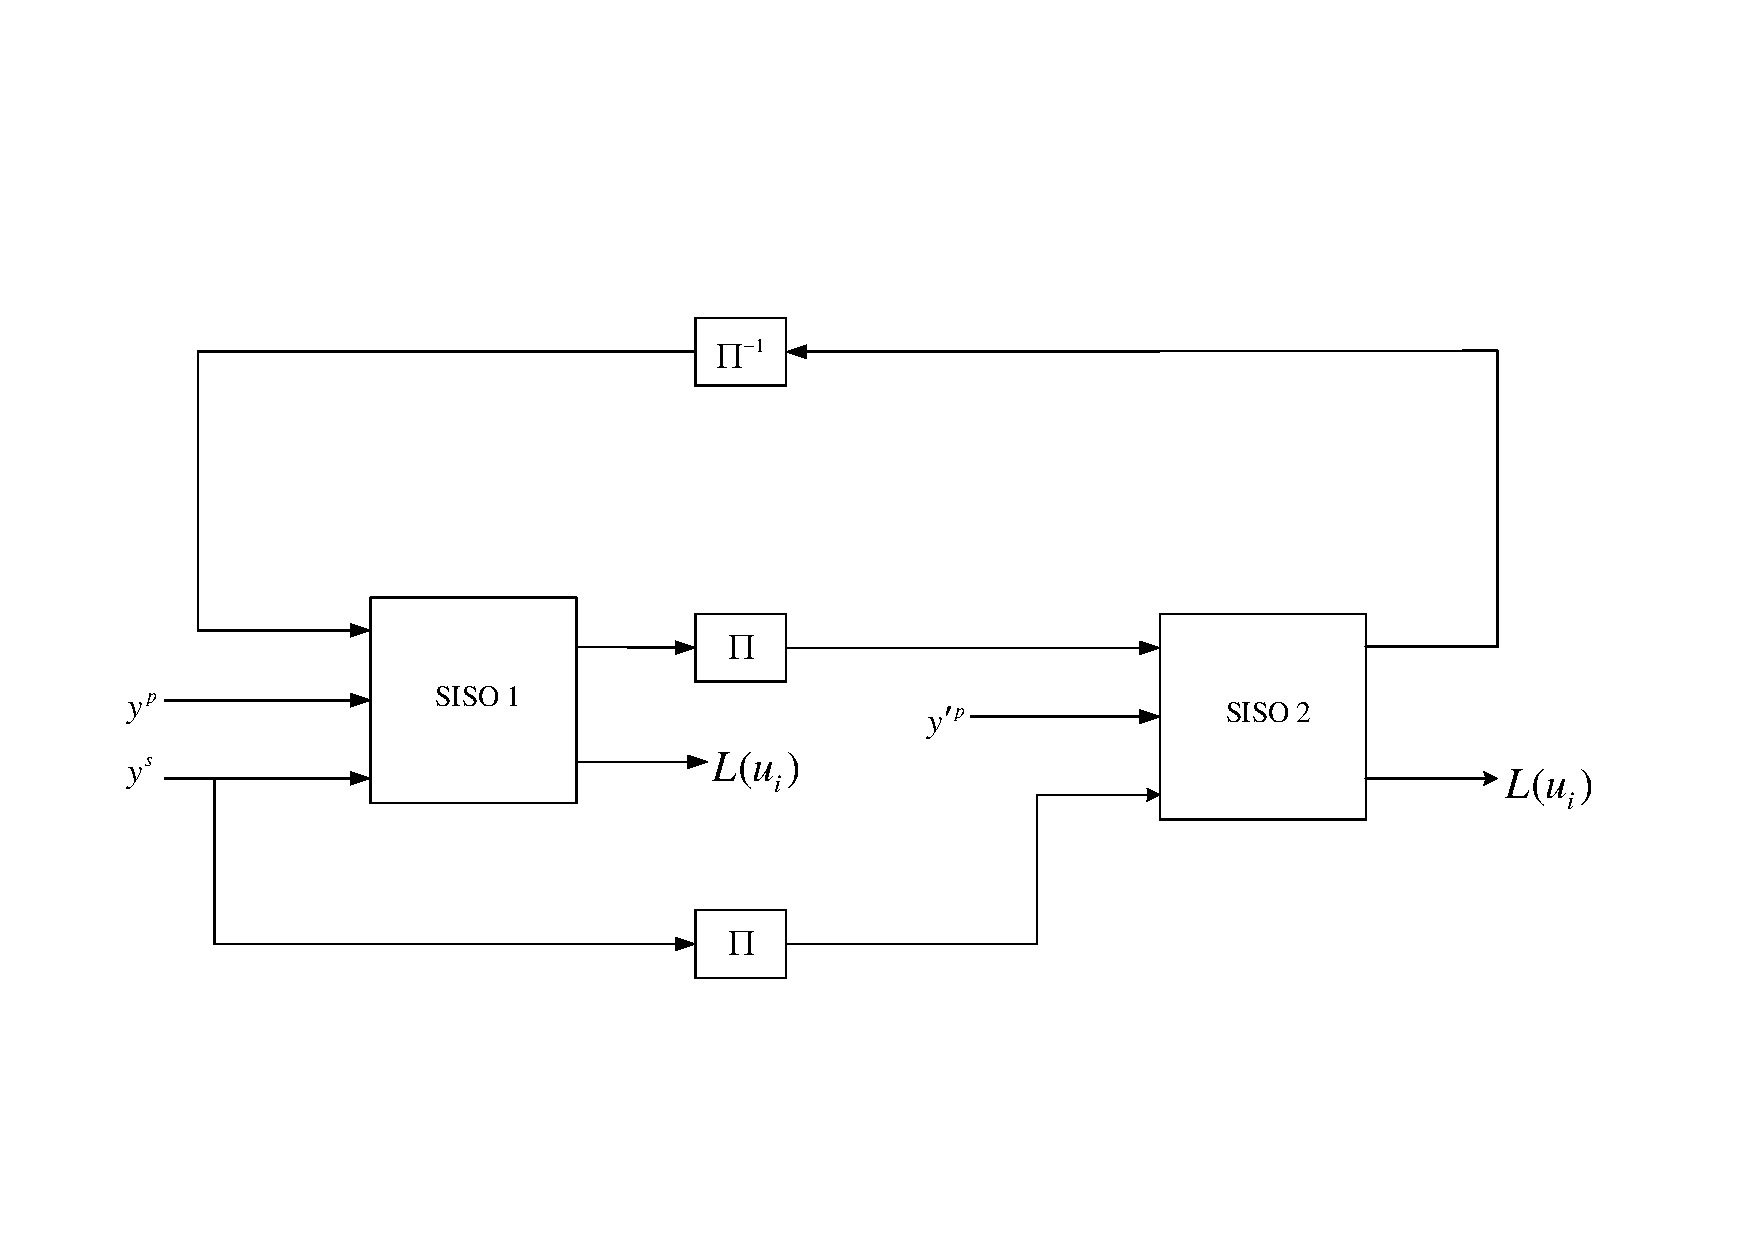
\includegraphics[width=0.45\textwidth]{D1.pdf}
		\caption{Turbo Decoder}
		\label{TDC}
		\end{figure}
	
 
 The system diagram for the turbo decoder is shown in figure (\ref{TDC}). It is made up of 2
 Soft Input Soft Output (SISO) decoders (one for each encoder). The decoding 
 process is carried out using turbo decoding algorithm which is based of the use of
 the BCJR algorithm or its variation.  The Max-Log-MAP algorithm is used 
 for its improved numerical stability and simplification of the calculations involved. 
 The algorithm is used to calculate the a posteriori Log-Likelihood Ratio (LLR),  
 $L(x_i|\mathbf{y})=\ln \frac{P(x_i=1|\mathbf{y})}{P(x_i=0|\mathbf{y})}$ 
 of the bits received. This also requires
 the calculation of state transition, feedfoward and feedback probabilities which we
 represent by the symbols $\gamma,\alpha, \beta $ respectively[from BCJR]. We 
 represent the previous trellis state and current trellis state by $\sigma'$ and $\sigma$ 
 respectively.
\begin{equation}
\begin{split}
&\gamma_i(\sigma',\sigma)=
\frac{x_i L_a (x_i)}{2}+
\frac{L_c}{2}\sum_{l=1}^{n} c_{i,l}y_{i,l}\,\,\,\,\, ,L_a(x_i) =\frac{P(x_i=1)}{P(x_i=0)}
\,\,\,\,\, ,Lc=4R_c\frac{E_b}{N_0}\\
&\alpha_i(\sigma)=\max_{\sigma'}[\alpha_{i-1}(\sigma')+\gamma_i(\sigma',\sigma)]\\
&\beta_i(\sigma')=\max_{\sigma}[\beta_{i}(\sigma)+\gamma_i(\sigma',\sigma)]
\end{split}
\label{abc}
\end{equation}
$c_i=\{x_i,p^{v}_i\}\,\,\,\, ,v=1,2$ and the initial values for $\alpha$ and $\beta$ are
\[
    \alpha_0(\sigma)= 
\begin{cases}
   0,& \sigma= 0\\        -\infty,              &  \sigma \neq 0
\end{cases}
\]

\[
   \beta_L(\sigma)= 
\begin{cases}
   0,& \sigma= 0\\        -\infty,              &  \sigma \neq 0
\end{cases}
\]
 \paragraph{}
$ L(x_i)$ is then calculated by using equation (\ref{LLR})
 \begin{equation}
 L(x_i)=\max_{R_1}[\alpha_{i-1}(\sigma')+ \gamma_i(\sigma',\sigma)+\beta_i(\sigma)]
 -
 \max_{R_0}[\alpha_{i-1}(\sigma')+ \gamma_i(\sigma',\sigma)+\beta_i(\sigma)]
\label{LLR}
\end{equation}
where $R_0,R_1$ are the subset of transitions caused by ''0'' and ''1'' respectively.



    
  The decoding process is as follows.
  

The input to the SISO1 is $\mathbf{y}^x,\mathbf{y}^{p^{(1)}}$ 
and $\mathbf{L}_a=\{L_a(x_0),L_a(x_1),...,L_a(x_{L})\}$. 
For the first iteration, it is assumed 
that the input information bits have equal probability and $\mathbf{L_a}$ is an 
all-zero vector.
These are used to calculate $\gamma ,\alpha , \beta$ using (\ref{abc})
 and finally
$ L(\mathbf{x})$ using (\ref{LLR}) and $\mathbf{L_e^{(1)}}$ is obtained by subtracting
 $L_c\mathbf{y}^x$  from each element in $ L(\mathbf{x})$ .
$\mathbf{L_e^{(1)}}$ is then
 interleaved and fed into SISO2 as the value for
 $\mathbf{L_a}$ along with an interleaved version of $\mathbf{y}^{x}$ and 
 $ \mathbf{y}^{p^{(2)}}$ which correspond to
 the interleaved systematic bits and the lower parity bits. These are used to calculate 
 $\gamma,\alpha , 
\beta, L(\mathbf{x})$
 and finally the extrinsic LLR values 
of the second component decoder, $\mathbf{L_e^{(2)}}$.
$\mathbf{L_e^{(2)}}$is deinterleaved、and fedback into the first component encoder
 as the new $\mathbf{L_a}$ value for SISO1.
\paragraph{}
The process is either repeated for a predetermined number of times, or untill a certain 
condition is met. At the final iteration $ L(\mathbf{x})$ (from the second component
 decoder) is deinterleaved and used to estimate the values of $\mathbf{x}$.
 
  It should be noted that, since CE2 was left open, 
 the final state at time $N-1$ could end up being any of the $2^m$ states with 
 probability $\frac{1}{2^m}$. Therefore in SISO2, the initial
 value of $\beta$, $\beta_L(\sigma)=-ln(2^m)$.

\section{Review of Linear Interleavers for Turbo Codes}
 RSC encoders are the component code of choice for turbo codes. They are
characterized by their cycle length ($\tau$) which is defined as the length of the cycle
 of the parity output of the encoder when the input $\mathbf{x}$ is $[1,0,0,0,....]$[PPI]. 
For example, the RSC encoder in figure (\ref{RSC})has a parity output $\mathbf{y}$ of 
$[1,1,1,0,1,1,0,1,1,0,...]$
for the previously mentioned input. As can be observed, the cycle is $[1,1,0]$ and
the cycle length $\tau=3$. With the knowledge of the cycle and the cycle length $\tau$
of the RSC encoder we wish to explore the effect of weight-2m inputs where the pair of
''1'' bits
 are seperated by $\tau-1$ ''0'' bits. We shall refer to to these inputs as
 $\tau$-seperated Weight-2m Input Error Events (or simply as $\tau$ weight-2m errors for
 simplicity sake ), where $m={1,2}$. 

\paragraph{}
 figure(\ref{RSC3})  shows the effect of $\tau$ weight-2 errors on the codeword weight.
 
\begin{figure}[h!]
\centering
		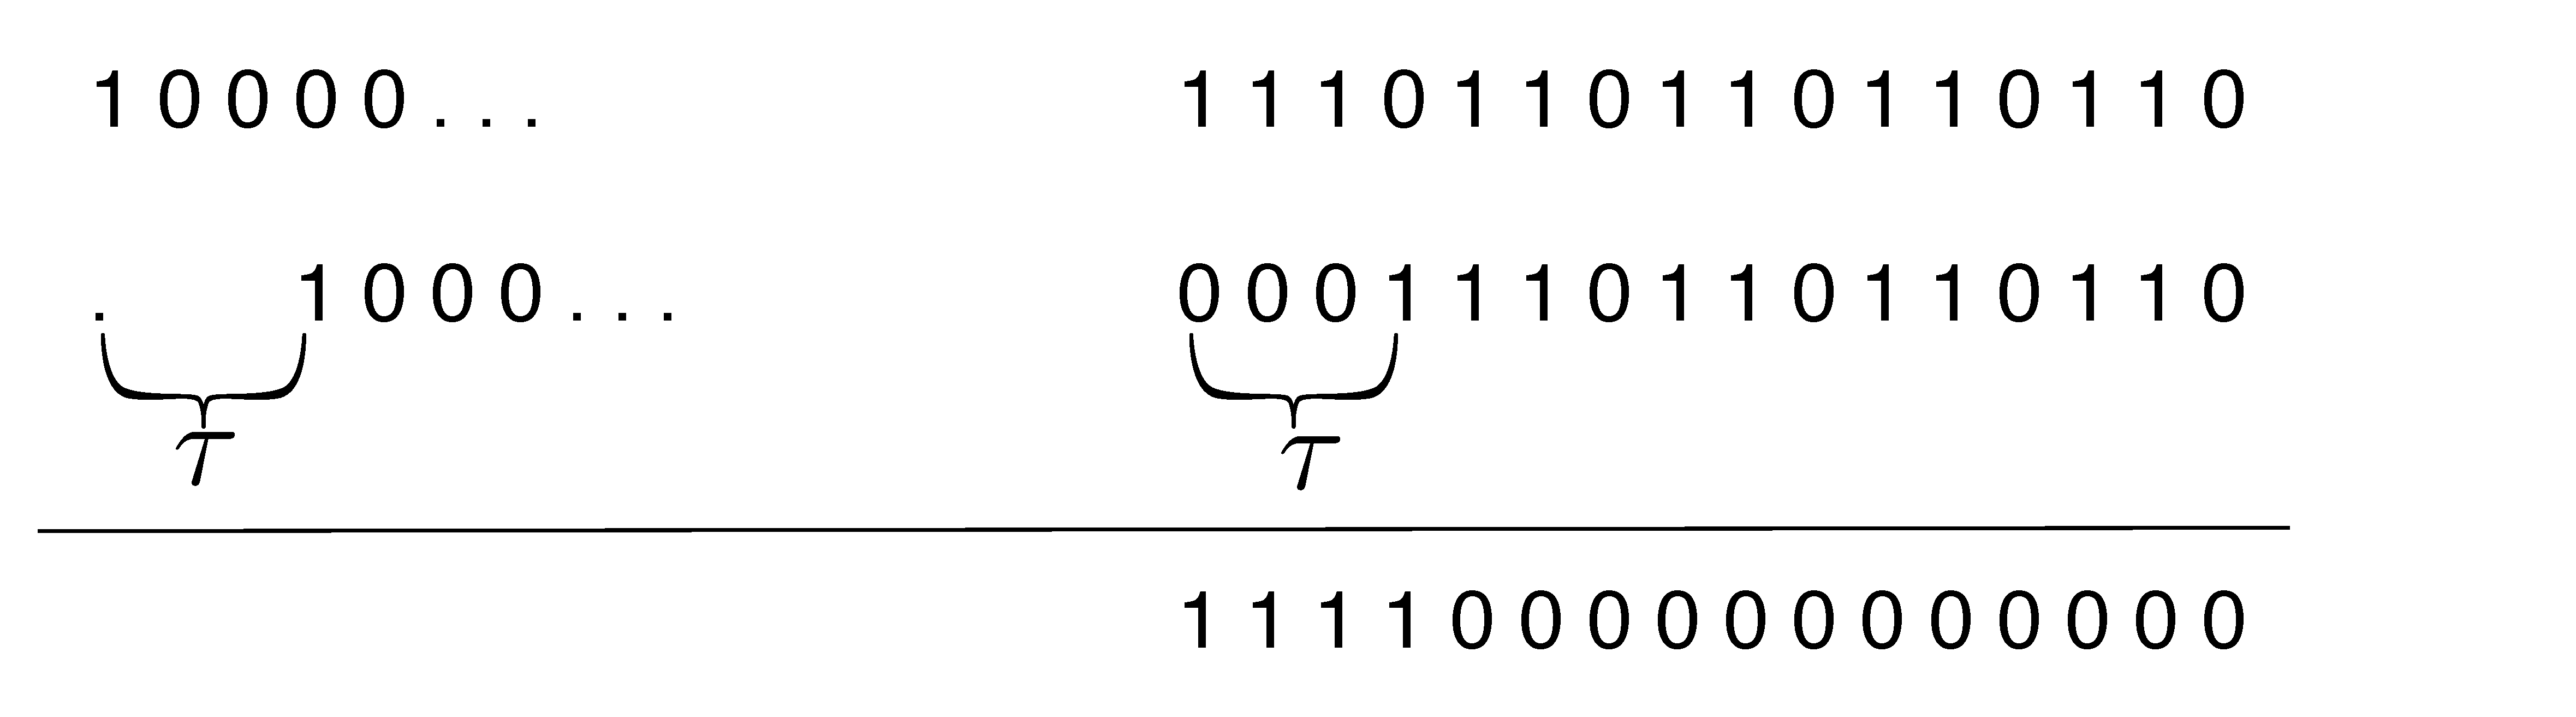
\includegraphics[width=0.45\textwidth]{RSCExample.pdf}
		\caption{ effect of $\tau$ weight-2 errors}
		\label{RSC3}
		\end{figure}
	
 The encoder used is the RSC encoder in figure (\ref{RSC})
  and the length N of this vector is assumed to 
be 16. The error vector may then be written as $[1, \mathbf{0}_{\tau-1} 1, \mathbf{0}_{N-\tau+1}]$
(where $\mathbf{0}_z$ is a zero vector of length z ).
This is equivalent to the modulo 2 addition of $\mathbf{x}$ and a version of
 $\mathbf{x}$ shifted by $\tau$ ,$\mathbf{x}_{\tau}$. As can be seen from 
figure(\ref{RSC3}) these inputs produce parity outputs $\mathbf{y}$ and $\mathbf{y}_{\tau}$
(version of $\mathbf{y}$ shifted by $\tau$). Modulo 2 addition of $\mathbf{y}$ and
$\mathbf{y}_{\tau}$ result in a low-weight parity output, which inturn results
in a low-weight parity codeword. It can easily be shown that a low-weight parity ouput
will be produced by $\tau$ weight-2 errors irrespective of position of the ''1'' bits . 
%In
%the case of $\tau$ weight-4 errors,the error vector may then be written as
 %$[1 ,\mathbf{0}_{\tau-1},1,\mathbf{0}_{u-1},1,\mathbf{0}_{\tau-1}
% ,1,\mathbf{0}_{N-(u+\tau)}]$ , where $u=2$.

 From the above example, we see that $\tau$ weight-2m errors have the potential to
produce low weight codeword with high multiplicity if they are present in both 
component encoders of the turbo encoder. This can be prevented by proper interleaver
 design.
 
The linear interleaver is a simple deterministic interleaver based on the circular shifting[2].
Its index mapping function is given by 
\begin{equation}
 \Pi_{\mathfrak{L}_N}(i) \equiv di \mod N \,\,\,\,\, 0 \leq i < N, \, gcd(N,d)=1
\end{equation}
From the mapping function, we can deduce that in an input sequence,
if there are 2 elements seperated by
a constant $t\mod N$ they will be mapped to an output sequence with the corresponding
elements seperated by a fixed constant $dt \mod N$. When used in turbo codes, there
exists a linear congruence relationship ( \ref{cong}) 
which is solvable and has a unique solution.
 \begin{equation} 
 dt \equiv \tau \mod N
 \label{cong}
 \end{equation}
where t is the distance between the ''1'' bits present in the weight-2 input.
For example for $N=32$, $d=5$ and component encoder in figure \ref{RSC}, 
$t=7$ satisfies the (\ref{cong}) . This means
that if the weight 2 input to the turbo code is of the form $(1+D^t)D^q,
\,\,\, q=0:N-t$ it is transformed
into a $\tau$ weight $2$ error. As long as the upper parity sequence has a large weight,
the codeword produced will most likely have a large weight. For weight $2$ inputs,
This is acheivable by 
carefully selecting the value of $d$ such that $t\neq a\tau,\,\,\, a=\{1,2,..\}$

The input weight $2$ analysis done above is a good method for ruling out bad interleavers.
However it is not sufficient for analyzing the performance of turbo codes at higher
$E_b/ N_o$. Doing analysis for higher input weights may offer deeper insights into
the performance of the turbo code, specifically weight $4$ inputs.

According to [2], weight 4 inputs of the form $(1+D^t)D^q+(1+D^t)D^{q+\tau}$
have the potential to produce low weight parity bits in both component codes. Using the 
same parameters as the previous example and assuming q=0, weight 4 inputs of the
form $1+D^7+D^3 +D^10$ which can be re-written as $1+D^3+D^7 +D^10$.
This is essentially 2 $\tau$ weight $2$ errors seperated by $t-\tau -1$ zeros. This input
is transformed into an input of the form $1+D^3+D^{15}+D^{18}$. The parity
bits for this input both have weight 8 and thus the total codeword weight is 20.
Though this value is large, the multiplicity of such codeword weights is approximately
N and therefore dominates the BER performance of the turbo code. Also changing the
size of the interleaver does not improve the performance.

In [6], the approximate expression for BER $P_e$ is derived and is given by
(\ref{aprox})
\begin{equation} 
 Pb(e) \approx \frac{1}{2}\sum_{w_c}D_{w_c} 
  erfc \Bigg(\sqrt{w_c\frac{R_cE_b}{N_o}} \Bigg)
  \label{aprox}
  \end{equation}
 where 
  $$ D_{w_c}\triangleq \sum_{w_x+w_p=w_c} \frac{w_x}{N}A_{w_x,w_p}$$
  $w_x$ is the weight of the input sequence, $w_p$ is the weight of the parity 
  sequence,$R_c$ is the rate of the turbo code , $w_c$ is the weight of the turbo 
  codeword and $A_{w_x,w_p}$ is the multiplicity of $w_c$. Using (\ref{aprox}),
  The BER curves are obtained for $\tau$ weight-2 and $\tau$ weight-4 errors. 
  This is shown in Figure (\ref{comp}). $N=1024$, $D=31$ and the component code used is the
  same as the one in Figure (\ref{RSC})
  The simulation results are also shown in the same graph. It can be observed that
  the approximation provided by the$\tau$ weight-2 error alone is largely over estimated,
  as the performance of the turbo code is clearly bound by  $\tau$ weight-4 error's
  curve. 
\begin{figure}[h!]
\centering
		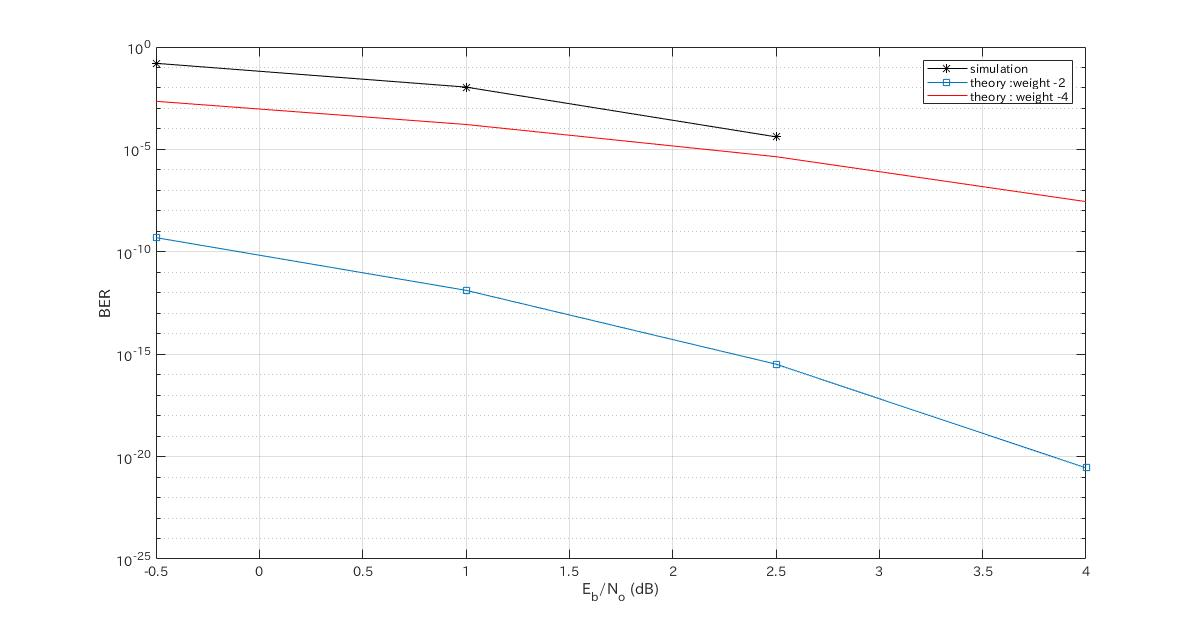
\includegraphics[width=0.45\textwidth]{D_31_N_1024_sim_VS_theory.png}
		\caption{Comparison of Linear interleaver BER performance: Simulation and Theoretical Results}
		\label{comp}
		\end{figure}





\section{Interleaver Design}
\label{sec}
In this section we present the design for a new deterministic interleaver. 
Our design is based on the idea of getting rid of the linear congruence
relationship to in order to get rid of the dominance of $\tau$ weight-4 errors
 . Guidlines for selecting
parameters to design good interleavers are presented.  
%$\tau$ weight-2m analysis is 
%carried out to confirm the resiliance of the new interleaver against  such errors.
 \subsection{Multi-Shift Interleaver}
 The process of linear interleaving is basically the shifting the positions of elements in
 a set by a certain factor d mod N and then use the following index mapping function.
 
 $$\Pi_{\mathit{L}_{N}} : x \mapsto L(p_x)\,\,\,\,\, 0\leq x<N$$
 
 The algorithm for the linear interleaver is shown below.
  
   1. $p_0=0$
 
  2. $p_i=p_{i-1}+d \mod N,\,\,\,\,\, 0<i<N,\,\,\, \mathit{d \,is \,an \,odd \,integer}$
 
 
 Keeping d constant along with the fact that gcd(d,N)=1 causes a linear congruence
  constraint 
 $$ dt \equiv \tau \mod N, \,\,\,\, $$. which in turn makes the
  linear interleaver succeptible to weight 4 inputs of the form 
  $(1+D^t)D^q+(1+D^t)D^{q+\tau}$
  \paragraph{}
  One possible method for getting rid of the linear congruence constraint is to increase
  the previous value of d by a value $\Delta s \mod N$  for every position shift . 
  It is shown in Example \ref{E1} and \ref{E2}
   that for $N=2^r,\,\,\, r=\{1,2,...\}$, changing the value of d for every shift still 
   causes
   the original sequence to be interleaved once d remains an odd number and $\Delta s$
   is an even number. By limiting the value of $\Delta s$ to $2^q,\,\,\, q=1:r-1$, we 
   have a set of d values which is of length of $N/\Delta s$. We shall refer to this 
   set as the cycle set. To maintain the idea of position shifting, the index mapping
   function used is of the form 
   $$\Pi_{\mathit{M}_{N:(d,\Delta s)}} : x \mapsto M(p_x)\,\,\,\,\, 0\leq x<N$$
  
  The algorithm for the proposed interleaver is shown below.
  
   1. $p_0=0$
 
 2a. $p_i=p_{i-1}+d \mod N,\,\,\,\,\, 0<i<N,\,\,\, \mathit{d \,is \,an \,odd \,integer}$
 
 2b. $d=\Delta s +d \mod N, \,\,\,\,\, \Delta s =2^q, \,\,\,\, q=1:r-1$
 
 
 \begin{example}
 \label{E1}
 : For $N=32$, the original set is $\{0,1,2,...,31\}$. The range of values for 
 $\Delta s = \{ 2,4,8,16\}$.  If we set the value
 of $\Delta s = 4$ and the initial value of $d=5$. 
 The cycle set is $\{ 5,9,13,17,21,25,29,1\}$ and the interleaved set is 
$\{0,5,30,27,12,1,10,23,24,29,22,19, 4, 25 ,2,15 ,16,21,\\14,11, 28,17,
  26, 7, 8, 13, 6, 3, 20, 9, 18, 31\}$
 \end{example}
 
  \begin{example}
  \label{E2}
 : For $N=32$, the original set is $[0,1,2,...,31]$. The range of values for 
 $\Delta s = \{ 2,4,8,16\}$.  If we set the value
 of $\Delta s = 8$ and the initial value of $d=5$. 
 The cycle set is $\{ 5,13,21,29\}$ and the interleaved set is 
  $\{0, 29, 18, 31, 4, 1, 22, 3, 8, 5, 26, 7, 12, 9, 30, 11, 16, 13, 2,\\
  15, 20, 17, 6, 19, 24, 21, 10, 23, 28,25, 14, 27\}$
 
 \end{example}
 It can be seen from the algorithm that the value of d as well as the position of the 
 elements of the set $x$ are shifted. We thus refer to this interleaver as the multi-shift 
 interleaver, which we shall denote by the symbol $\Pi_{\mathit{M}_{N:(d,\Delta s)}}$ .
 where d is the initial value in the cycle set.

 \subsection{Selecting Good Interleavers}
 For the proposed interleaver the parameters of importance are d and $\Delta s$ and
 by correctly choosing them we can design interleavers with performance better
 than the linear interleaver. 
  \paragraph{}
 The procedure we use for finding good interleavers is as follows. Assuming
 the interleaver length and the cycle length $\tau$ of the component 
 encoder is known, we first fix the value d and determine the elements of the cycle set.
 For each element in the cycle set, we calculate the hamming weight of the 
 turbo codewords 
 produced by $\tau$ weight-2 errors
 using the procedure in Figure \ref{RSC3} and record the minimum codeword weight. 

 
 The value of 
 $\Delta s$ that is chosen is the one that produces the largest minimum codeword 
 weight for $\tau$ weight-2 errors
 for a given value of d. In the case where the codeword weight is the same, the 
 multiplicity and $\Delta s$ are used as a tie breaker.
 
 It is essential to limit the range of d to search from adn we set it to
 odd integer values between $(\sqrt{N},N/2)$
 
 
 Table \ref{tab1} shows the best values of d, $\Delta s$
 as well as the value of the minimum weight codeword and its multiplicity($N_{free}$)
  for an interleaver 
 of length, $N=256$. The component encoder used is $\frac{1 + D^2}{1+D+D^2}$ 
 (octal notation: 5/7) 
 %and $\frac{1 +D+ D^2+ D^3+ D^4}{1+D^4}
  %$(octal notation: 37/21).
 
 \begin{table}[h!]
\centering
\begin{tabular}{||c |c |c |c||} 
 \hline
 d & 17 & 31 & 47 \\ [0.5ex] 
 \hline\hline
 $\Delta s(5/7)$ & 64 & 128 & 64 \\ 
 \hline
  $d_{eff}$ & 38 & 38 & 38 \\ 
  \hline
  $N_{free}$ & 207 & 208 & 209 \\ [1ex] 
 \hline
\end{tabular}
\caption{best value of d and corresponding value of $\Delta s$ 
and the value of the minimum weight codeword for
 turbo codes with $5/7$ $N=256$}
\label{tab1}
\end{table}

 Figure \ref{comp1} shows simulation results for Table 
 \ref{tab1}.
\begin{figure}[h!]
\centering
		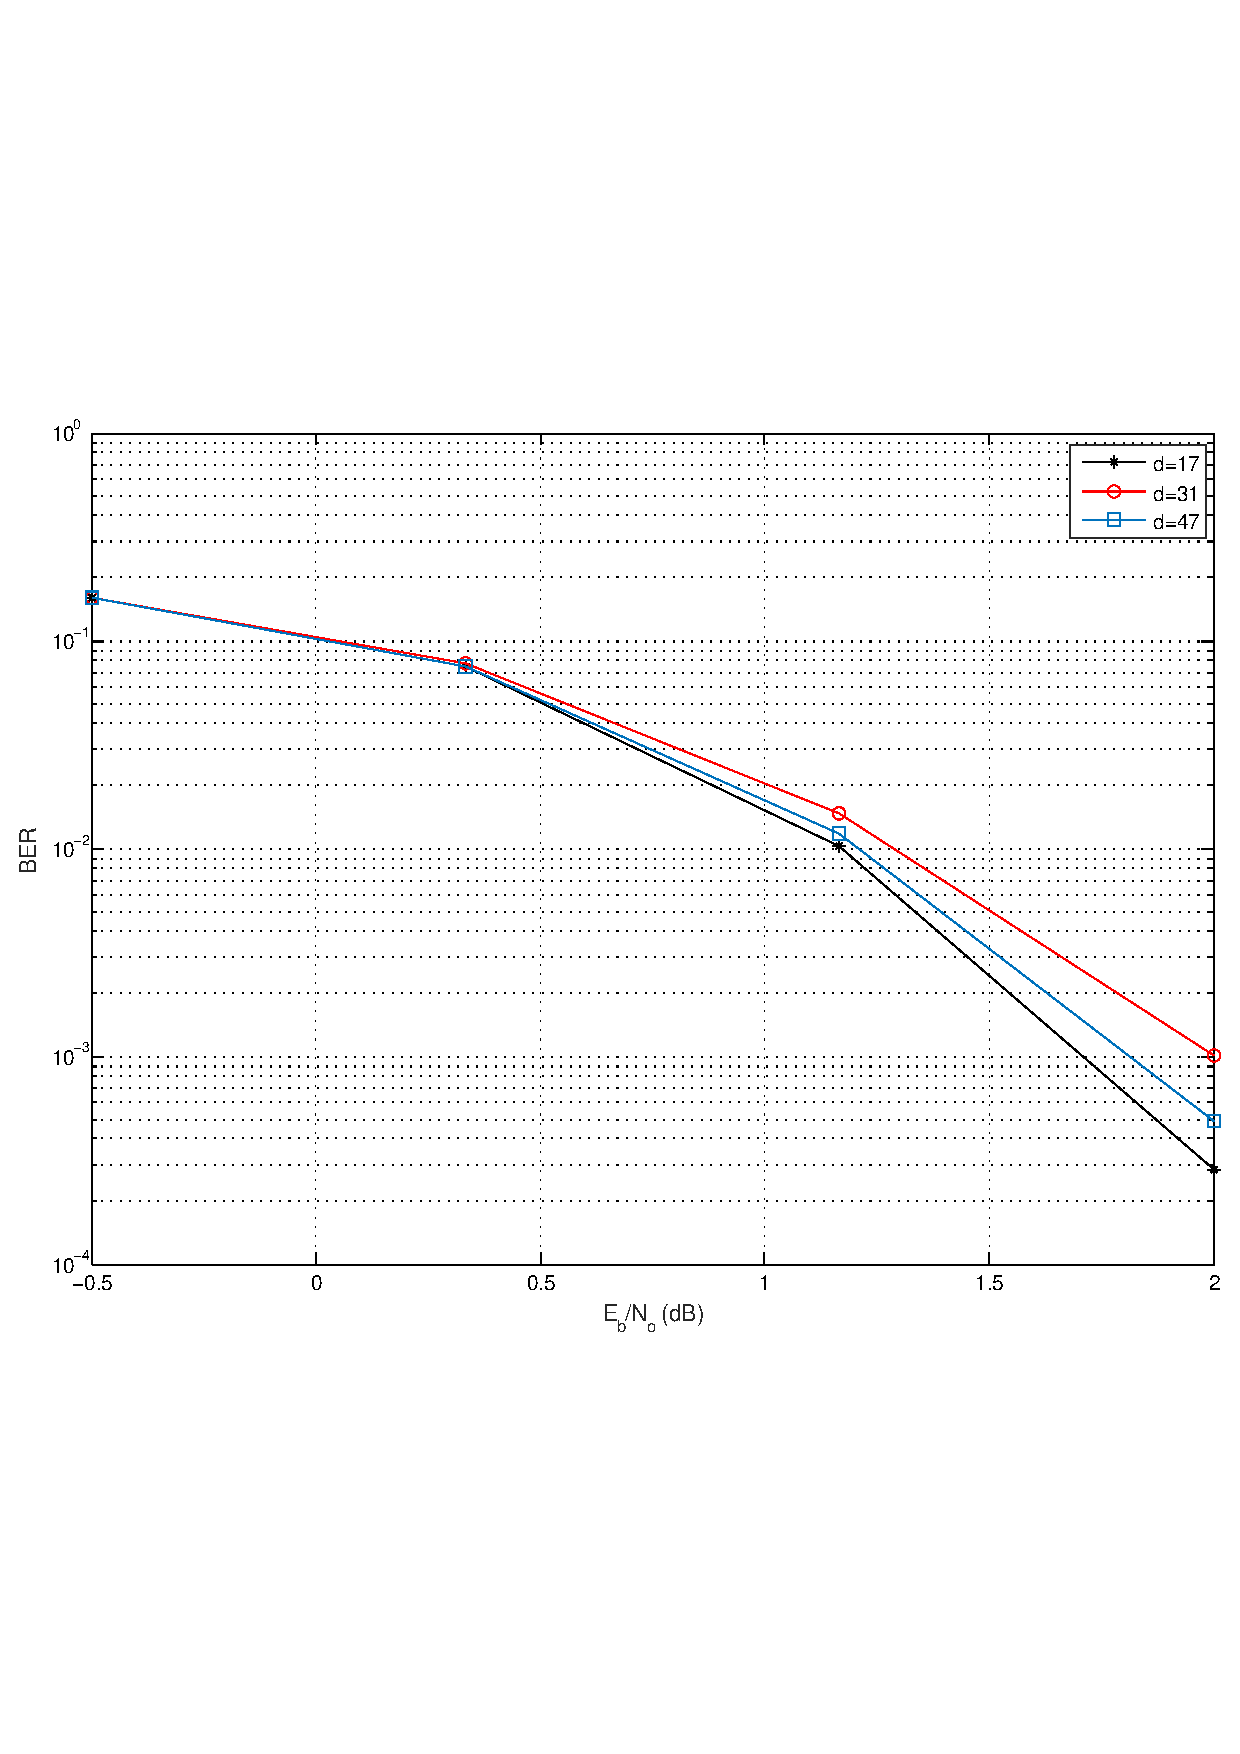
\includegraphics[height = 10 cm,width=0.45\textwidth]{myInterleaver_(comparison_256)_5_7_2.pdf}
		\caption{Simulation Results for Table \ref{tab1}}
		\label{comp1}
		\end{figure}
		
		%\begin{figure}[h!]
%\centering
	%	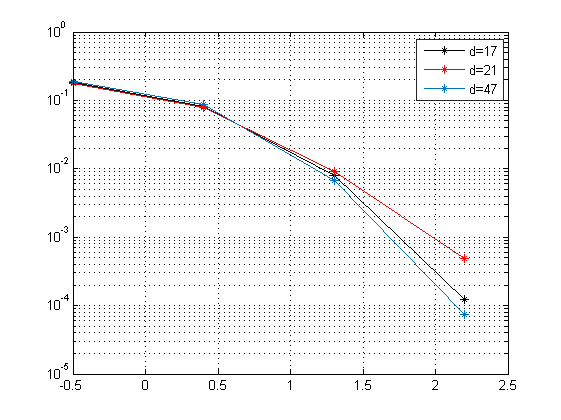
\includegraphics[width=0.75\textwidth]{comparison1.png}
		%\caption{Simulation Results for Table \ref{tab1}}
		%\label{comp2}
		%\end{figure}
\section{Results}
Given an Interleaver of size $N=2^r$ and component code, the search for good
multi-shift interleavers is an evaluation of the best combination of d and $\Delta s$.
 We  use the procedure outlined in Section \ref{sec}
to find the best value of $d$ and $\Delta s$. In this section, we present simulation 
results
for turbo codes designed using the multi-shift interleaver using different component
codes.
 Figure () and for  Figure () are the simulation results for the 5/7 component code
 and the 7/5 component code. The performance is compared with the Linear interleaver.
The interleaver length $N=1024$. In Figure (), the performance of the multi-shift 
interleaver is compared with the Linear interleaver  for the 
5/7 component code with interleaver length 16384
\section{Conclusion}

\section{References}
\paragraph{[1]}   John G. Proakis, Masoud Salehi. ''Digital Communications'', 
Fifth Edition,Chapter 8, McGraw-Hill.
\paragraph{[2]}  Oscar Y. Takeshita, Member, IEEE, and Daniel J. Costello ,
''New Deterministic Interleaver Designs for Turbo Codes'',IEEE Trans. Inform. 
Theory, vol.  46,pp. 1988-2006,Nov. 2000
\paragraph{[3]}  L. C. Perez, J. Seghers, D. J. Costello, Jr.,
 ''A distance spectrum interpretation of turbo codes'', IEEE Trans. Inform. Theory, 
 vol. 42, pp. 1698-1709, Nov. 1996.
\paragraph{[4]}  C. Berrou, A. Glavieux and P. Thitimajshima, 
''Near Shannon limit error-correcting coding and
decoding: Turbo codes'', Proc. Intern. Conf. Communications (ICC), Geneva, 
Switzerland, pp. 1064-
1070, May 1993. 
\paragraph{[5]}  Jing Sun, Oscar Y. Takeshita ''Interleavers for Turbo Codes Using 
Permutation Polynomials over Integer Rings'', IEEE Trans. Inform. Theory, vol. 51, 
pp. 101 - 119  Jan. 2005.
\paragraph{[6]} S. Benedetto and G. Montorsi, “Unveiling turbo codes: Some results
on parallel concatenated coding schemes,” IEEE Trans. Inform. Theory,
vol. 42, pp. 409–428, Mar. 1996.

\end{document}

% end of file
